\documentclass{article}

\usepackage{fancyhdr}
\usepackage{extramarks}
\usepackage{amsmath}
\usepackage{amsthm}
\usepackage{amsfonts}
\usepackage{tikz}
\usepackage[plain]{algorithm}
\usepackage{algpseudocode}
\usepackage{graphicx}
\usetikzlibrary{automata,positioning}
\usepackage{pdfpages}

%
% Basic Document Settings
%

\topmargin=-0.45in
\evensidemargin=0in
\oddsidemargin=0in
\textwidth=6.5in
\textheight=9.0in
\headsep=0.25in

\linespread{1.1}

\pagestyle{fancy}
\lhead{\hmwkAuthorName}
\chead{\hmwkClass\ (\hmwkClassInstructor\ \hmwkClassTime): \hmwkTitle}
\rhead{\firstxmark}
\lfoot{\lastxmark}
\cfoot{\thepage}

\renewcommand\headrulewidth{0.4pt}
\renewcommand\footrulewidth{0.4pt}

\setlength\parindent{0pt}

%
% Create Problem Sections
%

\newcommand{\enterProblemHeader}[1]{
    \nobreak\extramarks{}{Problem \arabic{#1} continued on next page\ldots}\nobreak{}
    \nobreak\extramarks{Problem \arabic{#1} (continued)}{Problem \arabic{#1} continued on next page\ldots}\nobreak{}
}

\newcommand{\exitProblemHeader}[1]{
    \nobreak\extramarks{Problem \arabic{#1} (continued)}{Problem \arabic{#1} continued on next page\ldots}\nobreak{}
    \stepcounter{#1}
    \nobreak\extramarks{Problem \arabic{#1}}{}\nobreak{}
}

\setcounter{secnumdepth}{0}
\newcounter{partCounter}
\newcounter{homeworkProblemCounter}
\setcounter{homeworkProblemCounter}{1}
\nobreak\extramarks{Problem \arabic{homeworkProblemCounter}}{}\nobreak{}

%
% Homework Problem Environment
%
% This environment takes an optional argument. When given, it will adjust the
% problem counter. This is useful for when the problems given for your
% assignment aren't sequential. See the last 3 problems of this template for an
% example.
%
\newenvironment{homeworkProblem}[1][-1]{
    \ifnum#1>0
        \setcounter{homeworkProblemCounter}{#1}
    \fi
    \section{Problem \arabic{homeworkProblemCounter}}
    \setcounter{partCounter}{1}
    \enterProblemHeader{homeworkProblemCounter}
}{
    \exitProblemHeader{homeworkProblemCounter}
}

%
% Homework Details
%   - Title
%   - Due date
%   - Class
%   - Section/Time
%   - Instructor
%   - Author
%

\newcommand{\hmwkTitle}{Homework\ \#8}
\newcommand{\hmwkDueDate}{Nov 10, 2019}
\newcommand{\hmwkClass}{CMSE 820}
\newcommand{\hmwkClassTime}{}
\newcommand{\hmwkClassInstructor}{Professor Yuying Xie}
\newcommand{\hmwkAuthorName}{\textbf{Boyao Zhu}}

%
% Title Page
%

\title{
    \vspace{2in}
    \textmd{\textbf{\hmwkClass:\ \hmwkTitle}}\\
    \normalsize\vspace{0.1in}\small{Due\ on\ \hmwkDueDate\ at 11:59pm}\\
    \vspace{0.1in}\large{\textit{\hmwkClassInstructor\ \hmwkClassTime}}
    \vspace{3in}
}

\author{\hmwkAuthorName}
\date{}

\renewcommand{\part}[1]{\textbf{\large Part \Alph{partCounter}}\stepcounter{partCounter}\\}

%
% Various Helper Commands
%

% Useful for algorithms
\newcommand{\alg}[1]{\textsc{\bfseries \footnotesize #1}}

% For derivatives
\newcommand{\deriv}[1]{\frac{\mathrm{d}}{\mathrm{d}x} (#1)}

% For partial derivatives
\newcommand{\pderiv}[2]{\frac{\partial}{\partial #1} (#2)}

% Integral dx
\newcommand{\dx}{\mathrm{d}x}

% Alias for the Solution section header
\newcommand{\solution}{\textbf{\large Solution}}

% Probability commands: Expectation, Variance, Covariance, Bias
\newcommand{\E}{\mathrm{E}}
\newcommand{\Var}{\mathrm{Var}}
\newcommand{\Cov}{\mathrm{Cov}}
\newcommand{\Bias}{\mathrm{Bias}}

\begin{document}

\maketitle

\pagebreak

\begin{homeworkProblem}
\textbf{Solution}\\
\begin{figure}
	\centerline{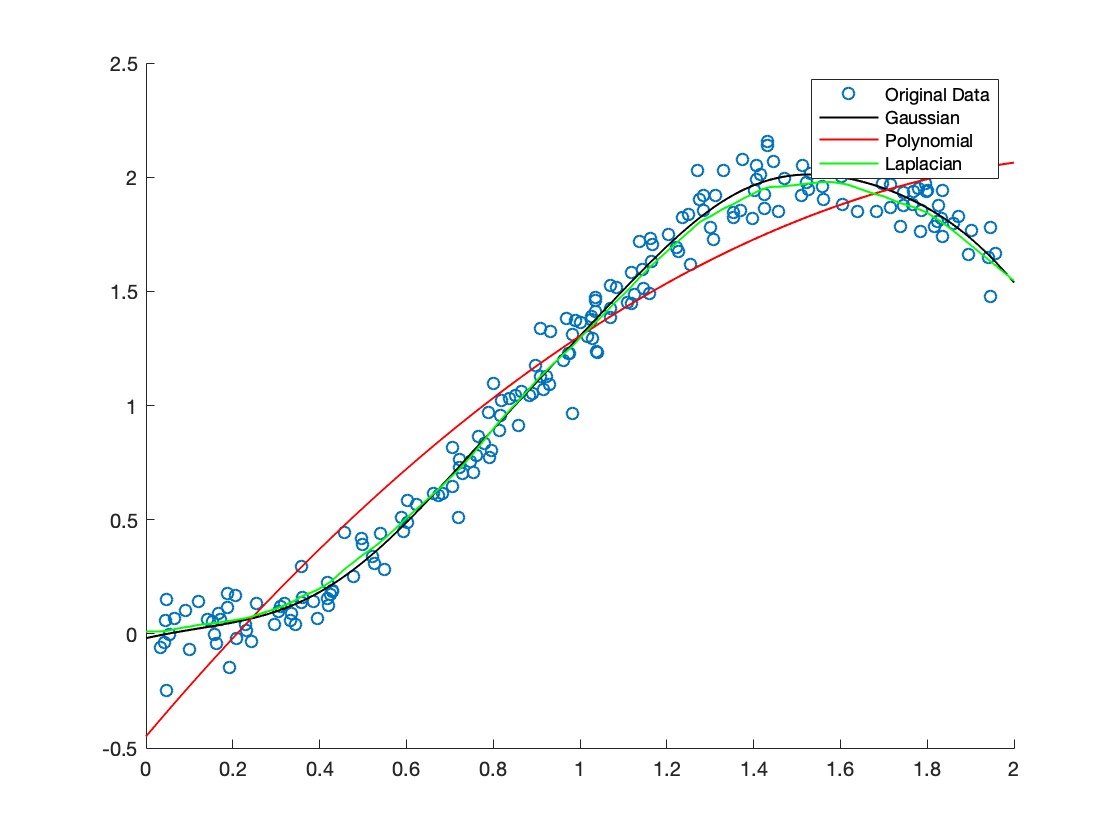
\includegraphics[scale=0.3]{untitled}}
	\caption{Plot of kernel regression functions $f(x)$ vs $x$ and original data}
\end{figure}
The plot is shown above.\\
The regression kernels and tuning parameter \(\lambda\) used are\\
(1) Gaussian kernel:  \(k(x,x') = \text{exp}(-\lVert x-x' \rVert^2/0.25)\) with \(\lambda\) = 0.01\\
(2) Polynomial kernel:  \(k(x,x') = (\langle x,x'\rangle + 1)^2 \text{ with } \lambda\) = 0.1\\
(3)Laplacian kernel:  \(k(x,x') = \text{exp}(-\lVert x-x'\rVert) \text{ with } \lambda\) = 1\\
\\
By comparing the RSS for the regression fit, we find that the quality of Gaussian kernel regression and Laplacian kernel regression is much better than that of Polynomial kernel regression.  We can explain this by noting that the feature maps of Gaussian kernel and Laplacian kernel map \(\mathcal{X}\) to an infinite dimensional space, while the feature map of the polynomial kernel is of a finite dimension.\\
\\
Residual(Gaussian) = 0.0079\\
Residual(Polynomial) = 0.0391\\
Residual(Laplacian) = 0.0081

\end{homeworkProblem}


\begin{homeworkProblem}
\textbf{Solution}\\
We perform binary classifications for pairs of 1, 2, 3, 4, i.e., \{1, 2\}, \{1, 3\}, \(\cdot\cdot\cdot\), \{3, 4\}. The data set for each pair is taken from the MNIST data set and split into two parts: training data set (60\%) and test data set (40\%).  RKHS ridge regression with the quadratic polynomial \(k(x,x') = (\langle x, x'\rangle + 1)^2\) is performed.  The tuning parameter \(\lambda\) is fixed at \(\lambda=10\) for simplicity.  

\begin{table}[h!]
\centering
 \begin{tabular}{||c c c c||} 
 \hline
  & 2 & 3 & 4 \\ [0.5ex] 
 \hline\hline
 1 & 99.70\% & 99.68\% & 99.81\% \\ 
 2 &  & 99.19\% & 99.73\% \\
 3 &  &  & 99.95\% \\[1ex] 
 \hline
 \end{tabular}
\end{table}


\end{homeworkProblem}


\begin{homeworkProblem}
\textbf{Solution}\\
Let \(\mathcal{B}=\{f_{\alpha}\in\mathcal{H}_k: f_{\alpha}=\sum_{i=1}^n\alpha_ik(x_i,\cdot),\alpha\in\mathbb{R}\) be a subspace of \(\mathcal{H}_k\).  Since \(\mathcal{B}\) is of finite dimension, \(\mathcal{B}\) is closed, and therefore \(\mathcal{H}_k=\mathcal{B}\oplus\mathcal{B}^{\perp}.\)  That is, \(\forall f\in\mathcal{H}_k\), there exists uniquely \(f_{\alpha}\in\mathcal{B}\) and \(f'\in\mathcal{B}^{\perp}\) such that \(f=f_{\alpha}+f'\).  Moreover, for any \(i = 1, \cdot\cdot\cdot, n,\) 
\[
f(x_i) = \langle f_{\alpha} + f', k(x_i,\cdot)\rangle = \langle f_{\alpha}, k(x_i, \cdot)\rangle = f_{\alpha}(x_i)
\]
Note also that, for any \(f\in\mathcal{H}_k, c[x_i, y_i, f(x_i)] = c[x_i, y_i, f_{\alpha}(x_i)],\) and
\[
\Omega(\lVert f\rVert_{\mathcal{H}_k}) = \Omega(\lVert f_{\alpha}+f'\rVert_{\mathcal{H}_k}) = \Omega(\sqrt{\lVert f_{\alpha}\rVert^2_{\mathcal{H}_k}+\lVert f'\rVert^2_{\mathcal{H}_k}})\geq\Omega(\lVert f_{\alpha}\rVert_{\mathcal{H}_k})
\]
So the minimizer \(\tilde{f}^\ast\in\mathcal{B}\oplus\) span\(\{\phi_j\}_{j=1}^m\subseteq\mathcal{F}\).  That is, there exists \(\alpha_i\in\mathbb{R}\) for all integers \(1\leq i\leq n\) and \(\beta_j\in\mathbb{R}\) for all integers \(1\leq j\leq n\) such that
\[
\tilde{f}^\ast  = \sum_{i=1}^n \alpha_i k(x_i,\cdot) + \sum_{j=1}^m\beta_j\psi_j
\]
Once \(\alpha\) is determined, the coefficient \(\beta\) can be found from
\[
\Psi\beta = \hat{Y}-\textbf{K}\alpha
\]
where \(\hat{Y} = (y_1,y_2,\cdot\cdot\cdot,y_n)\in\mathbb{R}^n, K_{ij}=k(x_i,x_j)\) and \(\Psi_{ij}= \psi_j(x_i)\).  Since \(\Psi\) is of full rank, it is invertible and \(\beta\) can be uniquely determined by
\[
\beta = \Psi^{-1}P_{\Psi}(\hat{Y}-textbf{K}\alpha) = (\Psi^T\Psi)^{-1}\Psi^T(\hat{Y}-\textbf{K}\alpha)
\]
\end{homeworkProblem}



\begin{homeworkProblem}
\textbf{Solution}\\
Is it obvious that \(\tilde{k}\) is symmetric by construction. (\(tilde{k}\) is well-defined when \(k(x,x)>0\) for all \(x\in\mathcal{X}.\))  For any positive integer \(N\in\mathbb{N}^+,\) for any real number \(c_i\in\mathbb{R}\), for any \(x_i\in\mathbb{X}\) where \(i = 1,\cdot\cdot\cdot,N\), we have
\[
\sum_{ij}c_ic_j\frac{k(x_i,x_j}{\sqrt{k(x_i,x_i)k(x_j,x_j}} = \sum_{ij}\Big(\frac{c_i}{\sqrt{k(x_i,x_i}}\Big)\Big(\frac{c_j}{\sqrt{k(x_j,x_j}}\Big)k(x_i,x_j)\geq 0
\]
The last inequality follows from the positive semi-definiteness of \(k\).  by the statement above, \(\tilde{k}\) is also p.s.d.
\end{homeworkProblem}



\begin{homeworkProblem}
\textbf{Solution 1.}\\
Solve
\[
\hat{f} = \underset{f\in\mathcal{H}}{\text{arg min}}\sum_{i=1}^n(y_i-f(x_i))^2+\lambda\lVert \omega\rVert^2, \quad (\ast)
\]

Let \(\Psi\) be an \(n\times N\) matrix such that \(\Psi_{ij}=\sqrt{\lambda_j}\psi_j(x_i)\) for \(i = 1,\cdot\cdot\cdot,n\) and \(j = 1,\cdot\cdot\cdot, N\) Define \(y = (y_1,y_2,\cdot\cdot\cdot,y_n)^T\in\mathbb{R}^n, \hat{y}=(f(x_1), f(x_2),\cdot\cdot\cdot, f(x_n))^T = \Psi\omega\in\mathbb{R}^n\).  We can rewrite the original problem as 
\[
\hat{\omega} = \underset{\omega\in\mathbb{R}^N}{\text{arg min}}\lVert Y - \Psi\omega\rVert^2 + \lambda\lVert \omega\rVert^2
\]
The corresponding Lagrangian is \(\mathcal{L}(\omega) = \lVert Y-\Psi\omega\rVert^2+\lambda\lVert\omega\rVert^2\).  Setting its partial derivative to 0 yields
\[
\frac{\partial \mathcal{L}}{\partial\omega} = -2\Psi^T(Y-\Psi\omega) + 2\lambda\omega = 0 \implies \hat{\omega}=(\Psi^T\Psi + \lambda \textbf{I})^{-1}\Psi^TY
\]
so \(\hat{f}=\sum_{j=1}^{N}\hat{\omega}_j\sqrt{\lambda_j}\psi_j\).
\\


\textbf{Solution 2.}\\
Recall the RKHS Ridge regression problem
\[
\hat{f} = \underset{f\in\mathcal{H}}{\text{arg min}}\sum_{i=1}^n(y_i-f(x_i))^2 + \lambda\lVert f\rVert^2_{\mathcal{H}} \iff \hat{\alpha} = \underset{\alpha\in\mathbb{R}^n}{\text{arg min}}\lVert Y - \textbf{K}\alpha\rVert^2 + \lambda\alpha^T\textbf{K}\alpha
\]
where \(\textbf{K}\) is an \(n\times n\) matrix such that \(\textbf{K}_{ij}=k(x_i,x_j)\).  The solution to this problem is given by 
\[
\hat{\alpha}=(\textbf{K}+\lambda\textbf(I))^{-1}Y
\]
Note also that by the Mercer's theorem
\[
\textbf{K} = \Psi\Psi^T
\]
We will show that the RKHS Ridge regression solution is also a solution to the problem (*).  Firstly, we need to show that the residual sums of squares are the same
\[
\begin{split}
&\lVert Y-\hat{Y}_{\hat{\alpha}}\rVert^2 = \lVert Y - \textbf{K}\hat{\alpha}\rVert^2 = \lVert Y-\Psi\hat{\omega}\rVert^2 = \lVert Y-\hat{Y}_{\hat{\omega}} \rVert\\
\iff &\textbf{K}\hat{\alpha} = \Psi\hat{\omega}\\
\iff &\textbf{K}(\textbf{K}+\lambda\textbf{I})^{-1}Y = \Psi(\Psi^T\Psi+\lambda\textbf{I})^{-1}\Psi^TY\\
\iff &\textbf{K}(\textbf{K}+\lambda\textbf{I})^{-1}-\Psi(\Psi^T\Psi+\lambda\textbf{I})^{-1}\Psi^T=0\\
\iff &\textbf{K} - \Psi(\Psi^T\Psi+\lambda\textbf{I})^{-1}\Psi^T(\textbf{K}+\lambda\textbf{I}) = 0\\
\iff &\textbf{K}-\Psi(\Psi^T\Psi+\lambda\textbf{I})^{-1}\Psi^T(\Psi\Psi^T + \lambda\textbf{I}) = 0\\
\iff &\textbf{K}-\Psi(\Psi^T\Psi+\lambda\textbf{I})^{-1}(\Psi^T\Psi + \lambda\textbf{I})\Psi^T = 0\\
\iff &\textbf{K}-\Psi\Psi^T = 0
\end{split}
\]
Secondly, we need to show that the penalty terms are equal as well.  Let \(\omega_{\hat{\alpha}}\) denote the corresponding \(\omega\) of the model \(\hat{\alpha}\) that satisfies \(f_{\hat{\alpha}} = \sum_j \omega_{\hat{\alpha}}\sqrt{\lambda_j}\psi_j(\cdot) = \sum_i\alpha_ik(\cdot,x_i)\).  In particular, considering the data points \(x_i\) only, we have \(\Psi\omega_{\hat{\alpha}}=\textbf{K}\alpha\).  Since \(\textbf{K}\hat{\alpha}=\Psi\hat{\omega}\)
\[
\Psi\omega_{\hat{\alpha}} = \Psi\hat{\omega} \Longrightarrow \omega_{\hat{\alpha}}=\hat{\omega} \Longrightarrow \lVert \omega_{\hat{\alpha}}\rVert = \lVert \hat{\omega}\rVert
\]
Thus, the model \(f_{\hat{\alpha}}\) given by \(\hat{\alpha}\) also solves the problem (\(\ast\)).  Since both the problem (\(\ast\)) and the RKHS Ridge regression problem are strictly convex optimization problems, so the solution is unique, implying that \(f_{\hat{\alpha}}=f_{\hat{\omega}}\) solves both of the problems.  Hence, the two problems are equivalent.



\end{homeworkProblem}


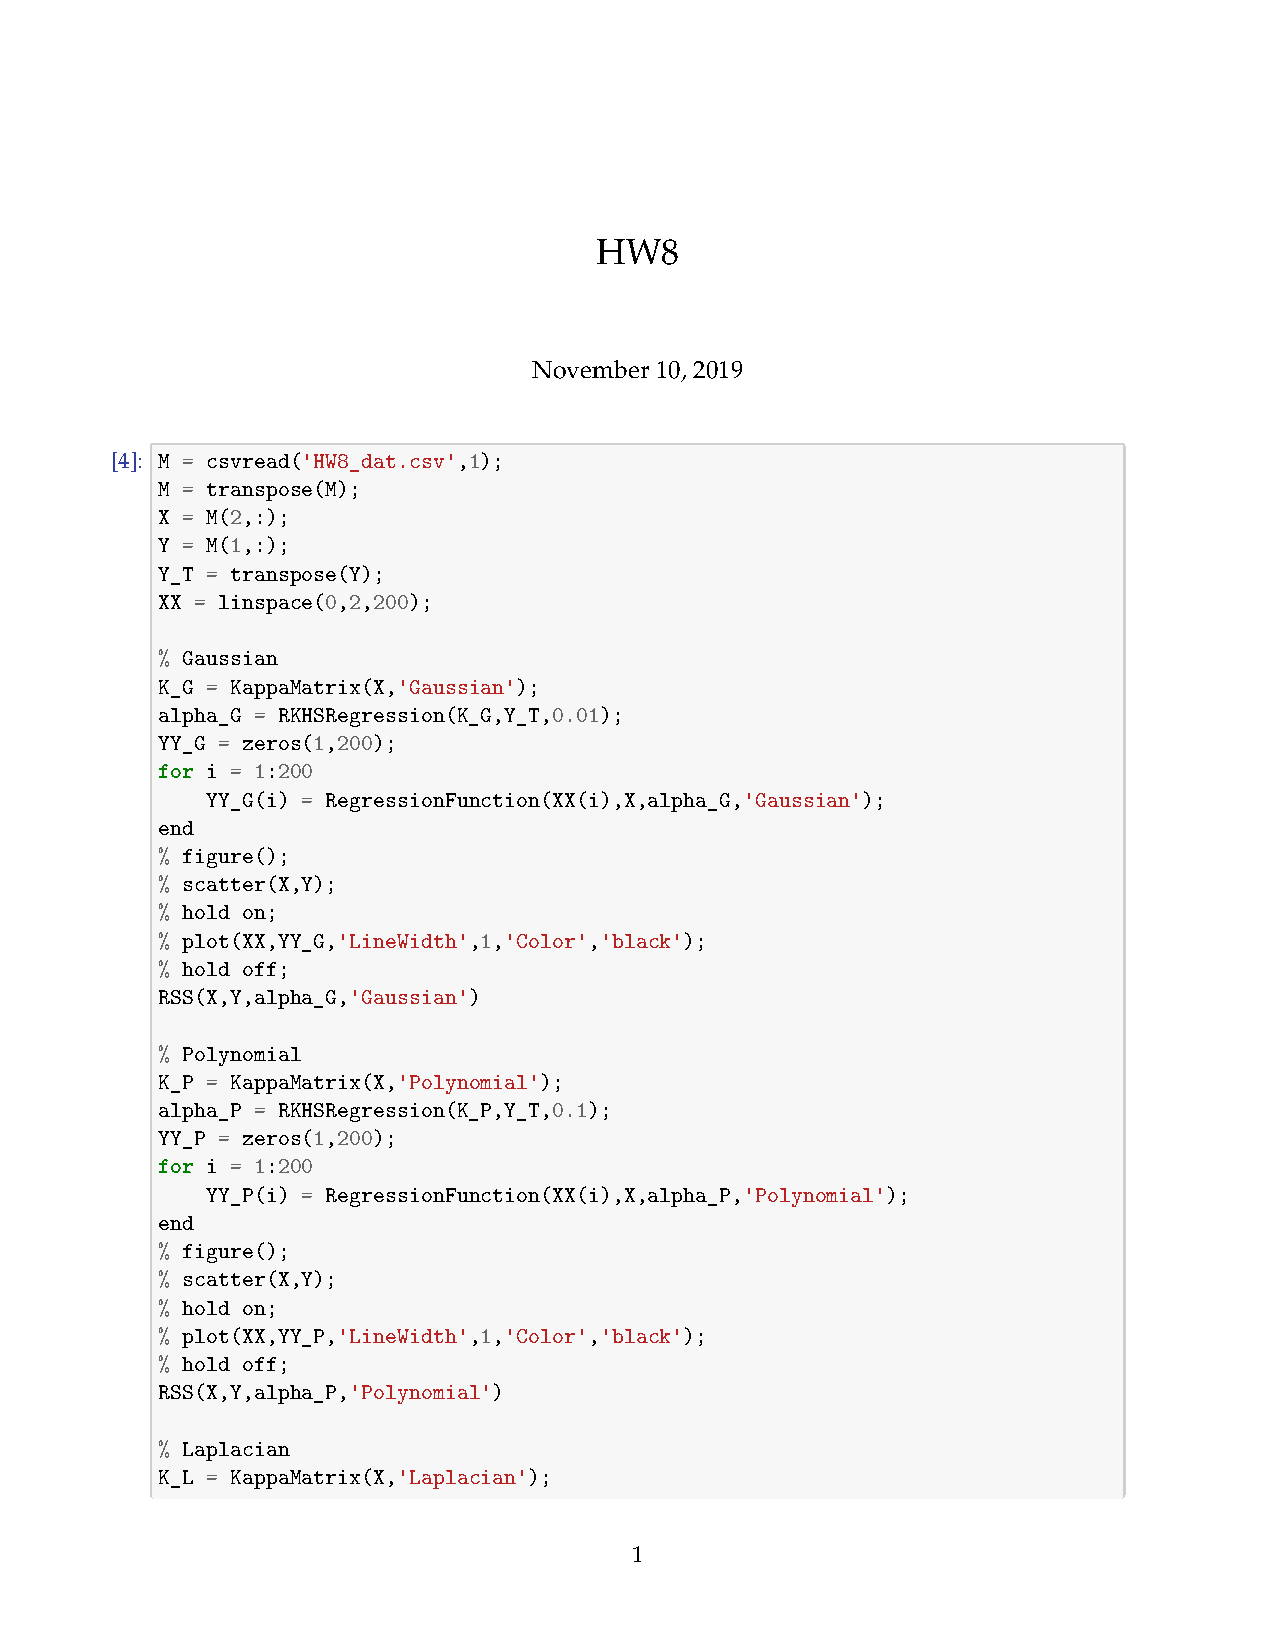
\includepdf[page={-}]{HW8_code.pdf}











\end{document}